\documentclass[11pt]{amsart}

\usepackage{amsmath}
\usepackage{physics}
\usepackage[utf8]{inputenc}
\usepackage{graphicx}

\title[Problem Sheet 10]{Problem Sheet 10\\
		\large{FYS3110}}
		
\author[Winther-Larsen]{Sebastian G. Winther-Larsen}

\date{\today}

\begin{document}

\maketitle

\section*{Problem 10.1}
The Zeeman correction, when choosing the external field $\vb{B}_{ext}$ to lie along the $z$-axis, can be expressed by the following condensed formula.
\begin{equation}
\label{eq:condensedzeeman}
E_Z^1 = \mu_B g_J B_{ext} j_z,
\end{equation}
where
\begin{equation}
\label{eq:bohrmagneton}
\mu_B = \frac{e\hbar}{2m} = 5.788\times10^{-5}eV/T
\end{equation}
is the Bohr magneton, and
\begin{equation}
\label{eq:langeg}
g_J=1 + \frac{j(j+1) + \frac{3}{4} - l(l+1)}{2j(j+1)}
\end{equation}
is the Landé g-factor. Adding the fine structure equation
\begin{equation}
\label{eq:finestructure}
E_{nj} = -\frac{13.6eV}{n^2}\left[1 + \frac{\alpha^2}{n^2} \left(\frac{n}{j + \frac{1}{2}} -\frac{3}{4} \right) \right]
\end{equation}
to the Zeeman correction (equation \ref{eq:condensedzeeman}) yields an equation for total energy in presence of weak-field Zeeman effect
\begin{equation}
\label{eq:totalweakzeeman}
E_{nljj_z} = -\frac{13.6eV}{n^2} \left[1 + \frac{\alpha}{n^2}\left(\frac{n}{j + \frac{1}{2}} -\frac{3}{4} \right) \right] + \mu_B g_J B_{ext} j_z.
\end{equation}

The weak-field Zeeman splitting for the first excited state of the hydrogen atom ($n=2$) is shown in figure  \ref{fig:weakzeemann2}. The energy $E_2$ is plotted against $\mu_BB_{ext}$ and we, evidently, get straight lines with slope $g_jj_z$, for every possible value of $j_z$. The energy splitting is very clear.

\begin{figure}
	\centering
	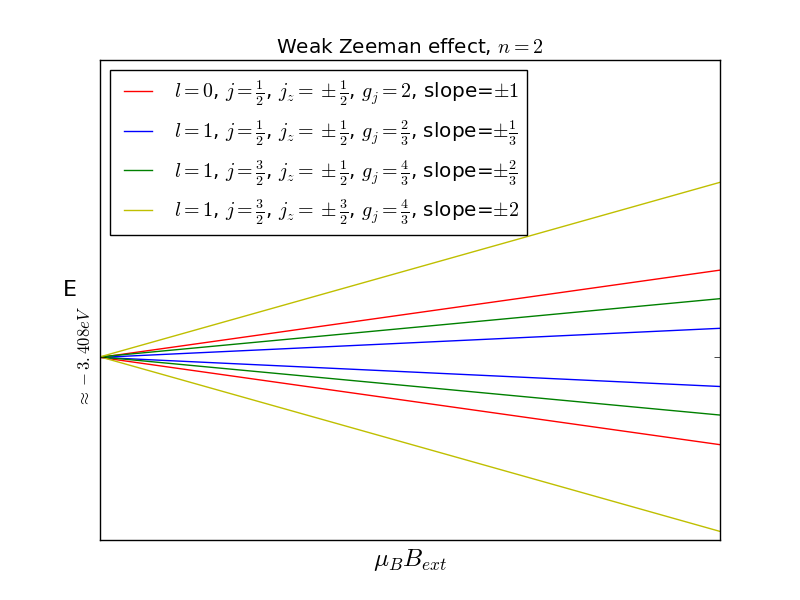
\includegraphics[width=0.9\textwidth]{figures/weakzeeman.png}
	\caption{Weak-field Zeeman splitting of the first excited state of hydrogen}
	\label{fig:weakzeemann2}
\end{figure}

\section*{Problem 10.2}

Assume that the proton of the hydrogen atom has finite size, in the shape of a sphere with radius $b=1\times10^{-15}m$. This would give it the proton an electric potential of
\begin{equation}
\label{eq:protonpotential}
V(r) = \begin{cases}
\frac{e}{4\pi\epsilon_0b}\left(\frac{3}{2} -\frac{r^2}{2b^2} \right), & r\leq b \\
\frac{e}{4\pi\epsilon_0r}, & r > b
\end{cases}
\end{equation}
and the electrostatic potential of an electron present in this potential would be $-eV(r)$. Unperturbed potential is $-\frac{e^2}{4\pi\epsilon_0r}$ which gives a perturbation of
\begin{equation}
\label{eq:perturbedhydrogenpot}
\Delta V(r) = \begin{cases}
-\frac{e^2}{4\pi\epsilon_0b}\left(\frac{3}{2}-\frac{r^2}{2b^2} \right) + \frac{e^2}{4\pi\epsilon_0r}, & r \leq b \\
\quad 0, & r > b.
\end{cases}
\end{equation}

The unperturbed ground state wave function for hydrogen is
\begin{equation}
\label{eq:unperturbedhydrogenground}
\ket{100} = \frac{1}{\sqrt{\pi a^3}}e^{-r/a},
\end{equation}
and the first order energy correction is
\begin{align*}
\Delta E	&= \bra{100}\Delta V(r)\ket{100} = \frac{1}{\pi a^3}\int_0^\pi\int_0^{2\pi}\int_0^b \Delta V e^{-2r/a}r^2\sin\phi dr dr\theta d\phi \\
			&= \frac{4\pi}{\pi a^3} \int_o^b \Delta V(r) e^{-2r/a} r^2 dr
\end{align*}
if $b << a$ then $e^{-2r/a}$, and we are left with
\begin{align*}
\Delta E	&= \frac{4}{a^3} \int_o^b \Delta V(r) r^2 dr = \frac{4}{a^3}\int_o^b -\frac{e^2 r^2}{4\pi\epsilon b} \left(\frac{3}{2} -\frac{r^2}{2b^2} \right) + \frac{e^2r^2}{4\pi\epsilon_0 r} dr \\
			&= \frac{4}{a^3}\frac{e^2}{4\pi\epsilon_0} \int_0^b -\frac{3r^2}{2b} + \frac{r^4}{2b^3} + r dr = \frac{4}{a^3}\frac{e^2}{4\pi\epsilon_0} \left(-\left[\frac{1}{2b}r^3 \right]_0^b + \left[\frac{1}{10b^3}r^5 \right]_0^b + \left[\frac{1}{2}r^2 \right]_0^b \right) \\
			&= \frac{4}{a^3}\frac{e^2}{4\pi\epsilon_0} \left(-\frac{1}{2}b^2 + \frac{1}{10}b^2 + \frac{1}{2}b^2 \right) = \frac{4}{5}\left(\frac{b}{a} \right)^2 \frac{e^2}{2(4\pi\epsilon_0)a}.
\end{align*}
Inserting for the Bohr radius, $a$, in the last fraction yields
\begin{equation}
\Delta E = \frac{4}{5}\left(\frac{b}{a}\right)^2\frac{m_e e^4}{2(4\pi\epsilon_0)^2\hbar^2}=\frac{4}{5}\left(\frac{b}{a}\right)^2Ry \approx 2.85 \times 10^{-10} Ry \approx 3.87 \times 10^{-9}eV 
\end{equation}

For comparison, the fine structure shift is (for $n=1$ and $j=\frac{1}{2}$)
\begin{equation*}
\Delta E_{fs} = 1.8088\times10^{-4}eV
\end{equation*}
and the hyperfine structure shift is
\begin{equation*}
\Delta E_{hs} = 5.88\times10^{-6}eV
\end{equation*}
One can see that the shift due to the perturbation of a finite-size proton is smaller than both the fine structure and hyperfine structure shift.

\section*{Problem 10.3}

The wave function for helium is the product of two hydrogen-like electron wave functions in 1s orbitals
\begin{equation}
\label{eq:heliumwave}
\psi_0(\vb{r}_1,\vb{r}_2) = \psi_{100}(\vb{r}_1)\psi_{100}(\vb{r}_2)=\frac{Z^3}{\pi a^3}e^{-Z(r_1+r_2)/a},
\end{equation}
and the helium Hamlitonian is
\begin{equation}
H = \frac{\hbar^2}{2m_e}(-\nabla^2_1-\nabla^2_2)\psi(\vb{r}_1,\vb{r}_2) - \frac{2e^2}{4\pi\epsilon_0}\left(\frac{1}{\vb{r}_1}+\frac{1}{\vb{r_2}} \right) + \frac{e^2}{4\pi\epsilon_0\abs{\vb{r}_2-\vb{r}_1}} = H^0 + H'
\end{equation}
The first order perturbative correction to the energy level is, as always
\begin{equation}
\label{eq:heliumgroundEpeturb}
E_n^1 = \bra{\psi_n^0}H'\ket{\psi_n^0}
\end{equation}
which, by inserting
\begin{equation*}
H' = \frac{e^2}{4\pi\epsilon_0\abs{\vb{r}_2-\vb{r}_1}},
\end{equation*}
gives
\begin{equation}
E_n^1 = \frac{e^2}{4\pi\epsilon_0}\left(\frac{Z^3}{\pi a^3} \right)^2\int\frac{e^{-2Z(r_1+r_2)}}{\abs{\vb{r}_2-\vb{r}_1}}d^3\vb{r}_1d^3\vb{r}_2 = \frac{5Z}{8a}\left(\frac{e^2}{4\pi\epsilon_0} \right) = -\frac{5Z}{4}E_h
\end{equation}
Thus the ground state with first order perturbation correction is
\begin{equation}
E_0 = E_0^0 + E_0^1 = -4E_h + \frac{5}{8}ZE_h = -\frac{11}{4}E_h = -74.8eV
\end{equation}
when inserting $Z=2$. Variational theory gives the same result.


\end{document}